\documentclass{beamer}
\usepackage{soul}
\usepackage{amsmath}
    \usepackage{amssymb}
    \usepackage{amsthm}
    \usepackage{amsfonts}
    \usepackage{braket}
\setbeamertemplate{navigation symbols}{}

\setbeamercolor{frametitle}{fg=black,bg=white}
\setbeamercolor{title}{fg=black,bg=yellow!85!orange}
\usetheme{AnnArbor}

\beamersetuncovermixins{\opaqueness<1>{25}}{\opaqueness<2->{15}}
\begin{document}
\title{A Survey of Quantum Learning Theory}
\author{Asim and Bhavishya}
\date{\today} 

\begin{frame}
\titlepage
\end{frame}

\begin{frame}\frametitle{Table of contents}\tableofcontents
\end{frame} 


\section{Introduction} 
\begin{frame}\frametitle{Introduction} 
\begin{itemize}
    \item  In recent years Machine Learning(ML) and Quantum computation(QC) have emerged as really successful technologies.  \pause
    \item  A Lot of ML is based on \textit{Heuristics}(i.e. not very mathematically rigorous) but this talk will focus on the theoretical side
    called ``Quantum Learning Theory"(QML) and describe main results involving QC in three main learning models. \pause
    \item  The learner will be quantum in QML, the data may be quantum
    \end{itemize}
    \begin{center}
\begin{tabular}{ |c|c|c| } 
 \hline
  &  Classical learner &  Quantum learner\\ 
  \hline
  Classical data & Classical ML & QML \\ 
  \hline
  Quantum data & ? &  QML \\ 
 \hline
\end{tabular}
\end{center}
 \end{frame}



\section{How can QC help ML?} 
\subsection{How can QC help ML?}
\begin{frame}\frametitle{How can QC help ML?}
\begin{itemize}
\item \textbf{Main Idea:} Inputs to ML problems are mostly 
high-dimensional vectors(imagine pixels for images, frequencies for audio etc.) i.e. $v \in \mathbb{R}^d$.
We can represent them using $\log($d) qubits,

$\Rightarrow$ $\ket{v}$ $=$ $\dfrac{\sum_{j=1}^{d} v_{i}\ket{j}}{||v||}$.

\item Then we can apply Quantum algorithms to learn from this efficient representation.
\item \textbf{Caveat:} Quantum Machine Learning algorithms provide an exponential speedup only under 
certain assumptions like existence of quantum RAM,  robustly invertible matrices etc. which make them 
difficult to implement in practice.

\end{itemize} 
\end{frame}

\begin{frame}\frametitle{Tools from QC}
\begin{itemize}
\item Grover Search: Provides sqrt speedup while searching unstructured databases
\item Fourier Sampling: Exponentially faster than classical Fourier Sampling.
% \item %TODO: Pretty good measurement
\end{itemize} 
\end{frame}


\begin{frame}\frametitle{Learning Models}
\begin{itemize}
\item \textbf{Concept:} A function $c:$ \{0,1\}$^{n} \rightarrow$ \{0,1\}.
\item \textbf{Goal:} Assume x $\in$ \{0,1\}$^{n}$ as a $n$ ``feature" vector, then our goal is to learn $c$ from small number
 of examples: (x, c(x))

\begin{figure}
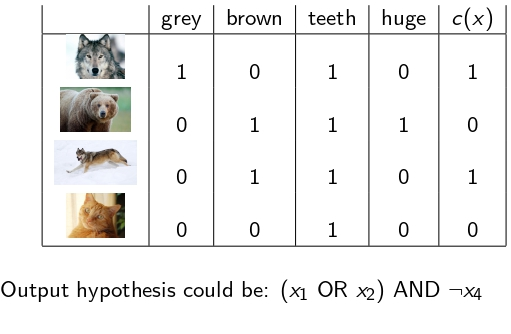
\includegraphics[scale=.9]{eg} 
\caption{Taken from Ronald de Wolf's talk}
\end{figure}

\end{itemize}
\end{frame}

\begin{frame}\frametitle{Formal definitions}
\begin{itemize}
\item \textbf{Concept:} some function $c:$ \{0,1\}$^{n} \rightarrow$ \{0,1\} 
\item \textbf{Concept class} $\mathcal{C}:$ set of all concepts( eg: DNFs with small number of terms)
\item Different types of learning

\begin{enumerate}
    \item Exact learning:  $\forall c \in \mathcal{C}$, given access to MQ(c) 
    oracle: w.p. $\geq 2/3$, output $h$ s.t. $h(x)=c(x)$ $\forall$ $x$  
    \item PAC learning: $\forall c \in \mathcal{C}$ and distribution $D$,given access to
    PEX($c, D$) orcale: w.p $\geq$ $1-\delta$, outputs $h$ s.t. Pr$_{x \sim   D}$ [$h(x) \neq c(x)$] $\leq \varepsilon$  
    \item Agnostic learning: $\forall$ distributions $D$ on \{0,1\}$^{n+1}$ 
    , given access to AEX(D) oracle: w.p. $\geq$ $1-\delta$, outputs $h \in \mathcal{C}$ s.t. err$_{D}(h) \leq opt_{D}(\mathcal{C}) + \varepsilon$
\end{enumerate}
 
\end{itemize}
\end{frame}


\begin{frame}\frametitle{Framework for measuring complexity of Learning}
\begin{itemize}
  \item    \textbf{Sample Complexity:} Number of examples used 
  \item    \textbf{Time Complexity:} Number of time-steps used 
\end{itemize} 



A good learner has small time and sample complexity, Next we compare Quantum and
Classical algorithms on the basis of their sample and time complexity.
\end{frame}


\begin{frame}\frametitle{VC dimension determines Sample Complexity}

\begin{itemize}
  \item  It characterizes the power of hypothesis class. Eg: Linear classifiers < Polynomial classifiers.
  \item Measured by ability to \textit{shatter} $n$ points. Shatter means to classify
  $n$ points in all possible labels.
  \item The max of $n$ is called the VC dimension of the hypothesis class.
  \item Hanneke'16 showed that for every concept class $\mathcal{C}$
  there exists an $(\varepsilon, \delta)$-PAC-learner using $O(\dfrac{VC}{\varepsilon} + \dfrac{\log(1/\delta)}{\varepsilon})$ examples
\end{itemize} 

\end{frame}




\begin{frame}\frametitle{Using Quantum Data}
\begin{itemize}
    \item We can put the classical data in a quantum 
    superposition 

    $  \sum_{x \in \{0,1\}^{n} } \sqrt{D(x)} \ket{x, c(x)} $

    \item Under uniform $D$ it is $ \dfrac{1}{\sqrt{2^{n}}} \sum_{x \in \{0,1\}^{n} }  \ket{x, c(x)} $

    \item Hadamard transformation changes this into $  \sum_{s \in \{0,1\}^{n} } \hat{c}(s) \ket{s} $
    where $\hat{c}(s) = \dfrac{1}{\sqrt{2^{n}}} \sum_{x} c(x) (-1)^{s.x}$ are the Fourier coefficients of
    $c$. This allows us to sample $s$  from distribution $\hat{c}(s)^{2}$.

    \item Eg: If $c$ is linear mod 2(c(x) = s.x for some s)
    then distribution peaks at s. Thus we can learn $c$ from one example.(Think Simon's algorithm)
    \item But in general PAC learning where $D$ can be any distribution
    quantum examples are not significantly better than classical examples [Arunachalam \& dW’17]
    
\end{itemize}

\end{frame}


\begin{frame}\frametitle{Proof sketch of lower bound}
\begin{itemize}
    \item %TODO:
\end{itemize}
\end{frame}

% \subsection{Pictures} 
% \begin{frame}\frametitle{pictures in latex beamer class}
% \begin{figure}
% \includegraphics[scale=0.5]{PIC1} 
% \caption{show an example picture}
% \end{figure}
% \end{frame}


\begin{frame}
\frametitle{Similar results for Agnostic Learning}
    \begin{itemize}
       \item Examples from unknown distribution $D$ on $(x, \ell)$. Predict
       $\ell$ from $x$, this allows us to model the case when 
       target concept might not even exist.

       \item Best concept from $\mathcal{C}$ has error \texttt{opt} = min$_{c \in \mathcal{C}}$ Pr$_{(x, \ell) \sim D}$ [$c(x) \neq \ell$]
       \item Therefor find $h \in \mathcal{C}$ with error $\leq$ \texttt{opt} + $\varepsilon$
       \item Classical Sample complexity: $T$ $= \Theta(\dfrac{VC}{\varepsilon^{2}} + \dfrac{\log(1/\delta)}{\varepsilon^{2}} )$
       \item By methods similar to PAC lower bound it can be shown that Qunatum Sample complexity is same as the classical case.
    \end{itemize}
\end{frame}


\begin{frame}
\frametitle{Quantum improvements in time complexity}
    \begin{itemize}
        \item Kearns \& Vazirani’94 gave a concept class 
        that is not efficiently PAC-learnable if factoring is hard

        \item But factoring is easy using Shor's algorithm. Therefore
        these classes can be learned efficiently[Servedio \&
        Gortler’04]

        \item Servedio \& Gortler’04: If classical one-way functions exist,
        then $\exists \mathcal{C}$ that is efficiently exactly learnable from membership
        queries by quantum but not by classical computers.
        Proof Idea: Use pseudo-random function to generate instances
        of Simon’s problem (special 2-to-1 functions). Simon’s
        algorithm can solve this efficiently, but classical learner would
        have to distinguish random from pseudo-random
    \end{itemize}
\end{frame}

\begin{frame}
\frametitle{Quantum improvements in time complexity}
    \begin{itemize}
        \item We can quadratic speedup for some ML problems
        and exponential speedup under \textit{very} strong assumptions.

        \item No improvements in Sample Complexity.
        \item Time complexity is exponentially improved for
        some concept classes like factoring.

        \item Various pragmatic issues like how to put big 
        classical data in superposition, issues with quantum memory.

    \end{itemize}
\end{frame}
\end{document}
